\PassOptionsToPackage{table,xcdraw}{xcolor}
\documentclass{beamer}

\definecolor{mybg}{RGB}{0,102,51}
\definecolor{emcolor}{RGB}{0,0,255}

\mode<presentation>
{
  \usetheme{Frankfurt}      % or try Darmstadt, Madrid, Warsaw, ...
  \usecolortheme{default} % or try albatross, beaver, crane, ...
  \usefonttheme{default}  % or try serif, structurebold, ...
  \setbeamertemplate{navigation symbols}{}
  \setbeamertemplate{caption}[numbered]
  \setbeamertemplate{footline}[frame number]
} 

% beamer stuff
%\useoutertheme[subsection=false]{smoothbars}
%\useinnertheme[shadow=true]{rounded}
%\usecolortheme{seagull}
%\setbeamerfont{block title}{size={}}
%\usefonttheme[onlylarge]{structurebold}
%\setbeamerfont*{frametitle}{size=\normalsize,series=\bfseries}
%\setbeamertemplate{navigation symbols}{}
%\setbeamercolor*{normal text}{fg=white,bg=gray}
%\setbeamercolor*{alerted text}{fg=white}
%\setbeamercolor*{example text}{fg=white}
%\setbeamercolor*{structure}{fg=white}
\AtBeginSection[]
{
  \begin{frame}%<beamer>
    \frametitle{Content}
    \tableofcontents[currentsection,currentsubsection,hideothersubsections]
  \end{frame}
}
% packages
\usepackage{enumerate}
\usepackage[table,xcdraw]{xcolor}
\usepackage{amssymb}
\usepackage{multicol}
\usepackage[normalem]{ulem}
\usepackage{wasysym}
\usepackage{listings}
\lstset{ %
  language=prolog,
%  frame=l,                   			% adds a frame around the code
  basicstyle=\scriptsize\ttfamily,	% use courier
  breaklines=false,
  xleftmargin=0em,
  aboveskip=0.5em,
  belowskip=0.5em,
%  belowcaptionskip=5em,
  numbers=left,
  backgroundcolor=\color{lightgray},
  frame=single,
  framerule=0pt
}
\usepackage{multimedia}
\usepackage{multirow}

% tikz stuff
\usepackage{tikz}
\usetikzlibrary{shadows}
\usetikzlibrary{shapes}
\usetikzlibrary{arrows}
\usetikzlibrary{calc}
\usetikzlibrary{fit}
\usetikzlibrary{backgrounds}
\usetikzlibrary{positioning}
\usetikzlibrary{chains}
\usetikzlibrary{scopes}
\usetikzlibrary{decorations}
\usetikzlibrary{decorations.text}
\usetikzlibrary{decorations.pathmorphing}
\usepackage{animate}

\usepackage{amsmath}
% \usepackage{paralist}

\newcommand{\myemph}[1]{{\bf {\color{emcolor}{#1}}}}

\begin{document}

\title{Evaluating CLEMI}
\subtitle{CLustering to Evaluate Multiple Imputation}
\author{\myemph{Anthony Chapman} \\ \and Dr Steve Turner \and Dr Wei Pang \and Dr Lorna Aucott}
% \author[S.\,Cauvin \& D.\,Sleeman \& W. \,Vasconcelos]
% {%
%   \texorpdfstring{
%       \begin{columns}%[onlytextwidth]
%           \column{.38\linewidth}
%           \centering
%           \myemph{Samuel Cauvin}\\
%           \href{mailto:s.cauvin@abdn.ac.uk}{s.cauvin@abdn.ac.uk}
%           \column{.2\linewidth}
%           \centering
%           Derek Sleeman\\
%           \href{mailto:d.sleeman@abdn.ac.uk}{d.sleeman@abdn.ac.uk}
%           \column{.38\linewidth}
%           \centering
%           Wamberto Vasconcelos\\
%           \href{mailto:w.w.vasconcelos@abdn.ac.uk}{w.w.vasconcelos@abdn.ac.uk}
%       \end{columns}
%   }
%   {Samuel Cauvin \& Derek Sleeman \& Wamberto Vasconcelos}
% }`'
\institute{
Dept. of Applied Medical Sciences, University of Aberdeen \\Dept. of Computing Science, University of Aberdeen \\e-mail: \href{mailto:r01ac14@abdn.ac.uk}{r01ac14@abdn.ac.uk}
}

\date{
\includegraphics[height=1cm]{logo}\hfill
\includegraphics[height=1cm]{logo-farr}}
% \logo{
\includegraphics[height=1cm]{logo}\vspace{205pt}} % logo on ever slide
\maketitle

\begin{frame}
  \frametitle{Outline}
  \tableofcontents
\end{frame}

\section{Testing Dataset 1}
\subsection{}

\begin{frame}
  \frametitle{Forest Fires Summary}
  Forest Fires:
  \begin{itemize}
    \item 517 records, 13 variables
    \item Mixed numerical and categorical variables
    \item Will select $x\%$ of records randomly 
    \item Will remove a random amount of variables from the selected records
    \item Chosen increments of 10\% (10\%-90\%)
  \end{itemize}
\end{frame}

\begin{frame}
  \frametitle{Evaluation ctn.}
  % Distance Measure:
  % \begin{itemize}
  %   \item Clustering characteristics 
  %   \item 
  % \end{itemize}
  \center{ 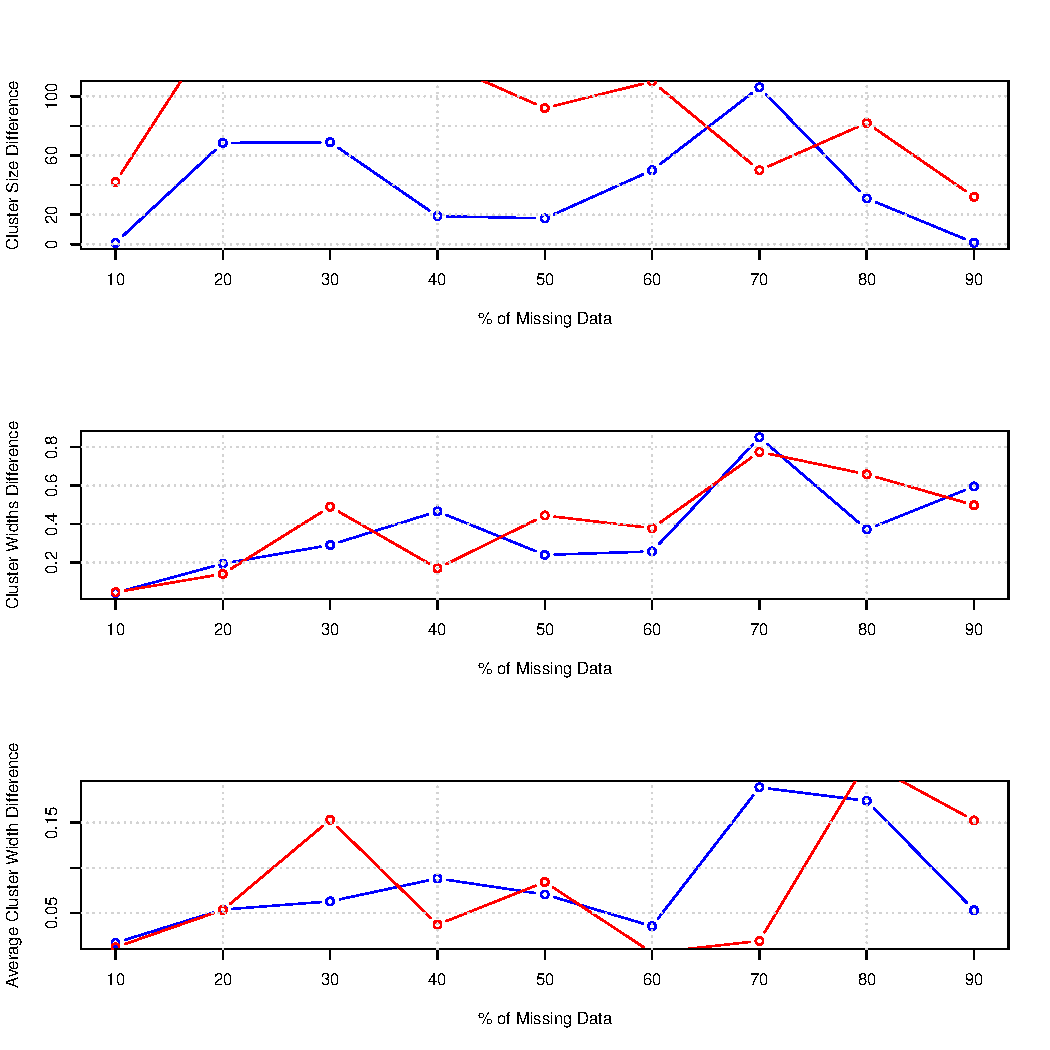
\includegraphics[width=\textwidth,height=0.9\textheight,keepaspectratio]{forestFires1} }
\end{frame}

\begin{frame}
  \frametitle{Evaluation ctn.}
  % Distance Measure:
  % \begin{itemize}
  %   \item Clustering characteristics 
  %   \item 
  % \end{itemize}
  \center{ 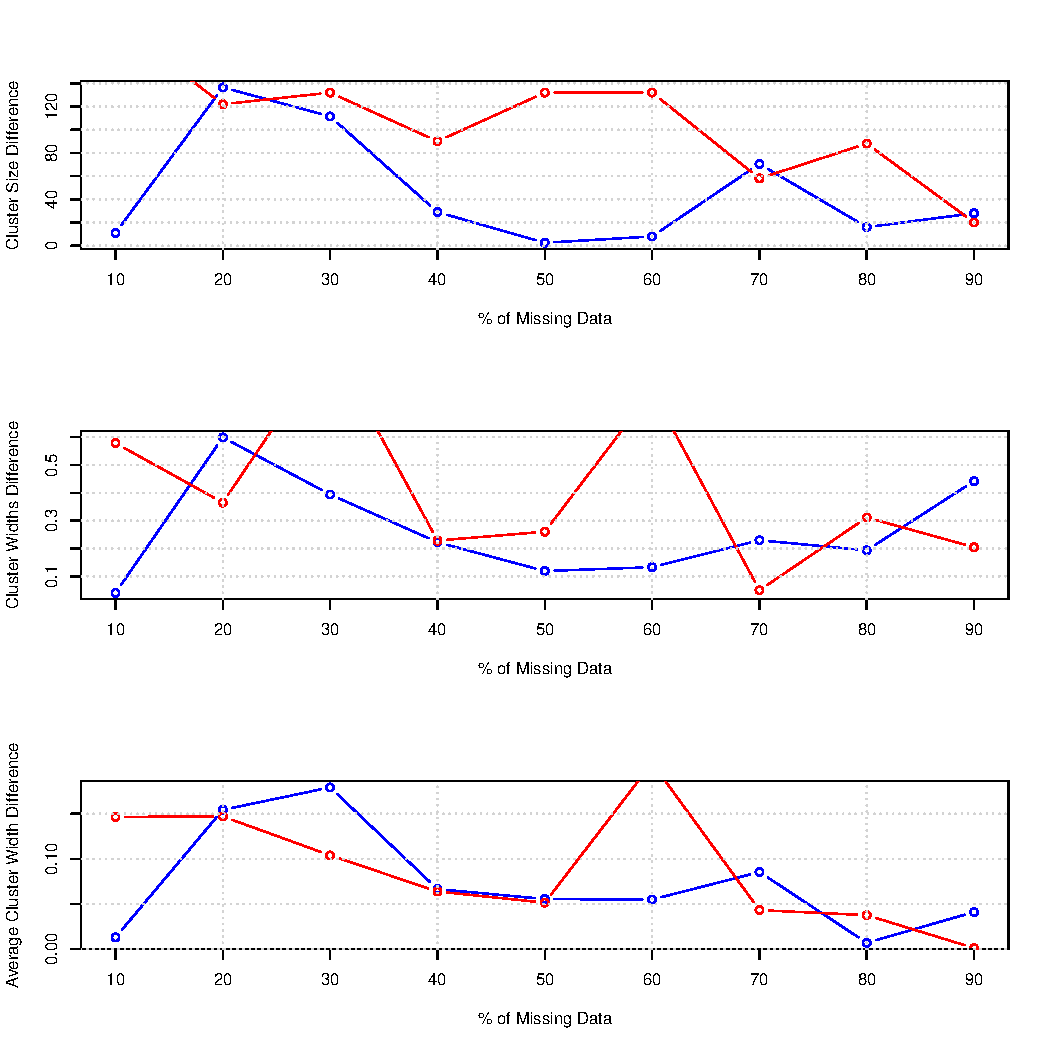
\includegraphics[width=\textwidth,height=0.9\textheight,keepaspectratio]{forestFires2} }
\end{frame}

\begin{frame}
  \frametitle{Evaluation ctn.}
  % Distance Measure:
  % \begin{itemize}
  %   \item Clustering characteristics 
  %   \item 
  % \end{itemize}
  \center{ 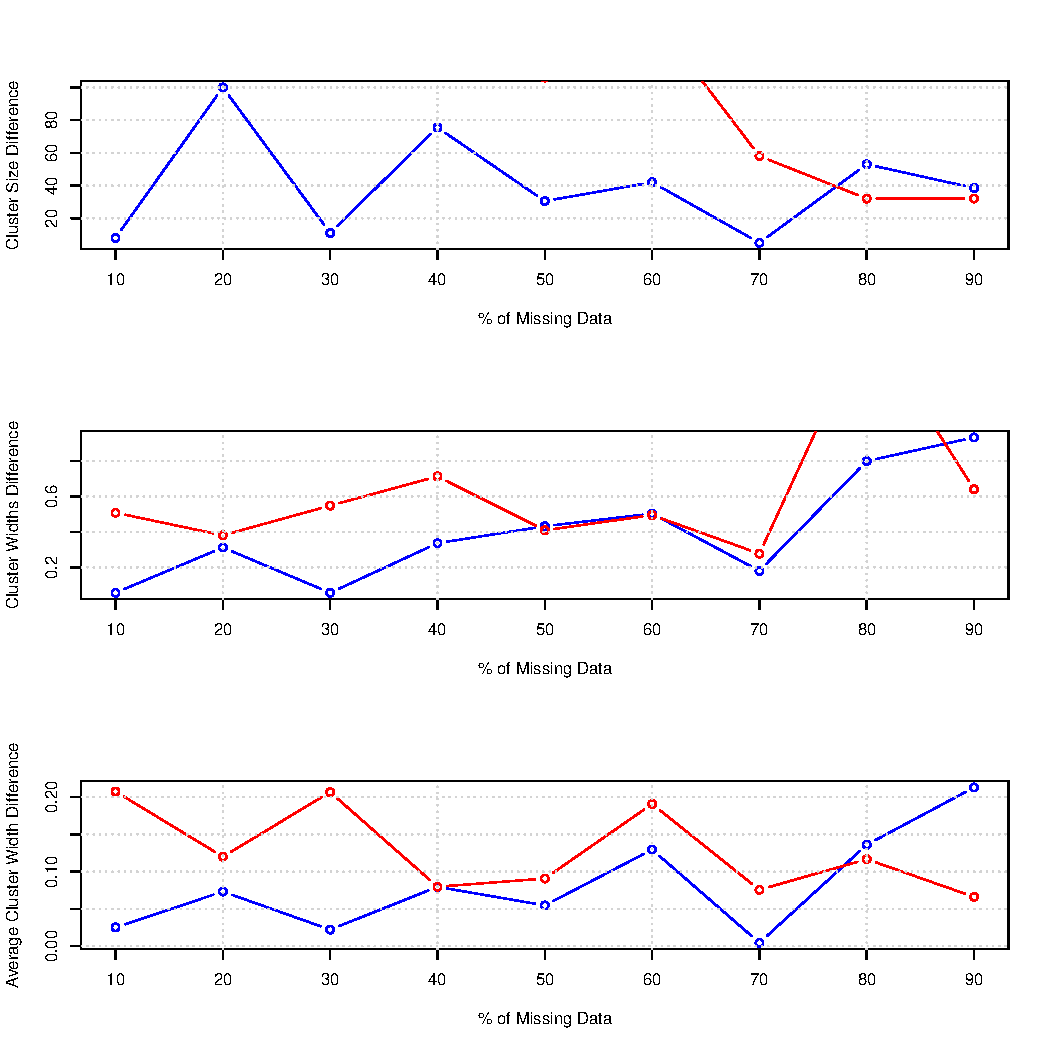
\includegraphics[width=\textwidth,height=0.9\textheight,keepaspectratio]{forestFires3} }
\end{frame}

\begin{frame}
  \frametitle{Evaluation ctn.}
  % Distance Measure:
  % \begin{itemize}
  %   \item Clustering characteristics 
  %   \item 
  % \end{itemize}
  \center{ 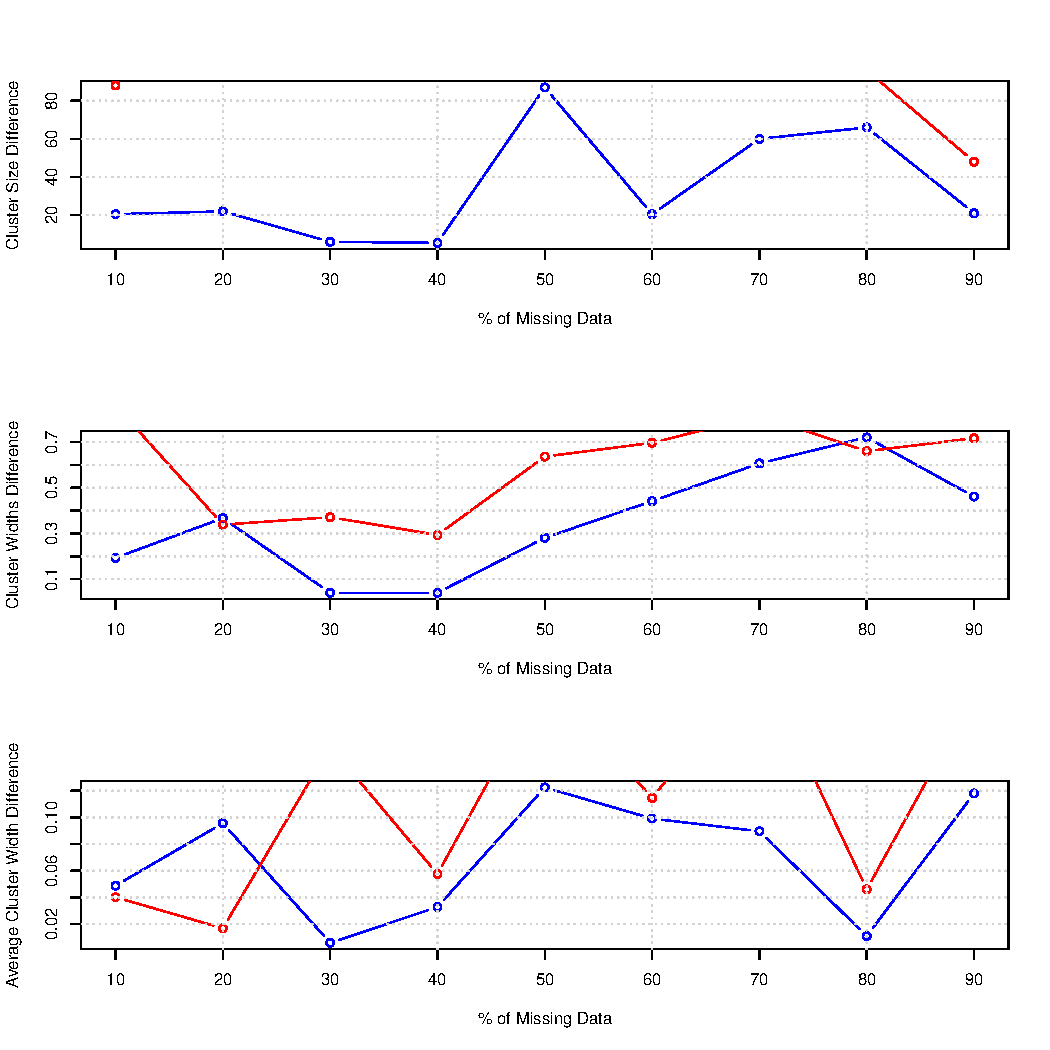
\includegraphics[width=\textwidth,height=0.9\textheight,keepaspectratio]{forestFires4} }
\end{frame}

\begin{frame}
  \frametitle{Evaluation ctn.}
  % Distance Measure:
  % \begin{itemize}
  %   \item Clustering characteristics 
  %   \item 
  % \end{itemize}
  \center{ 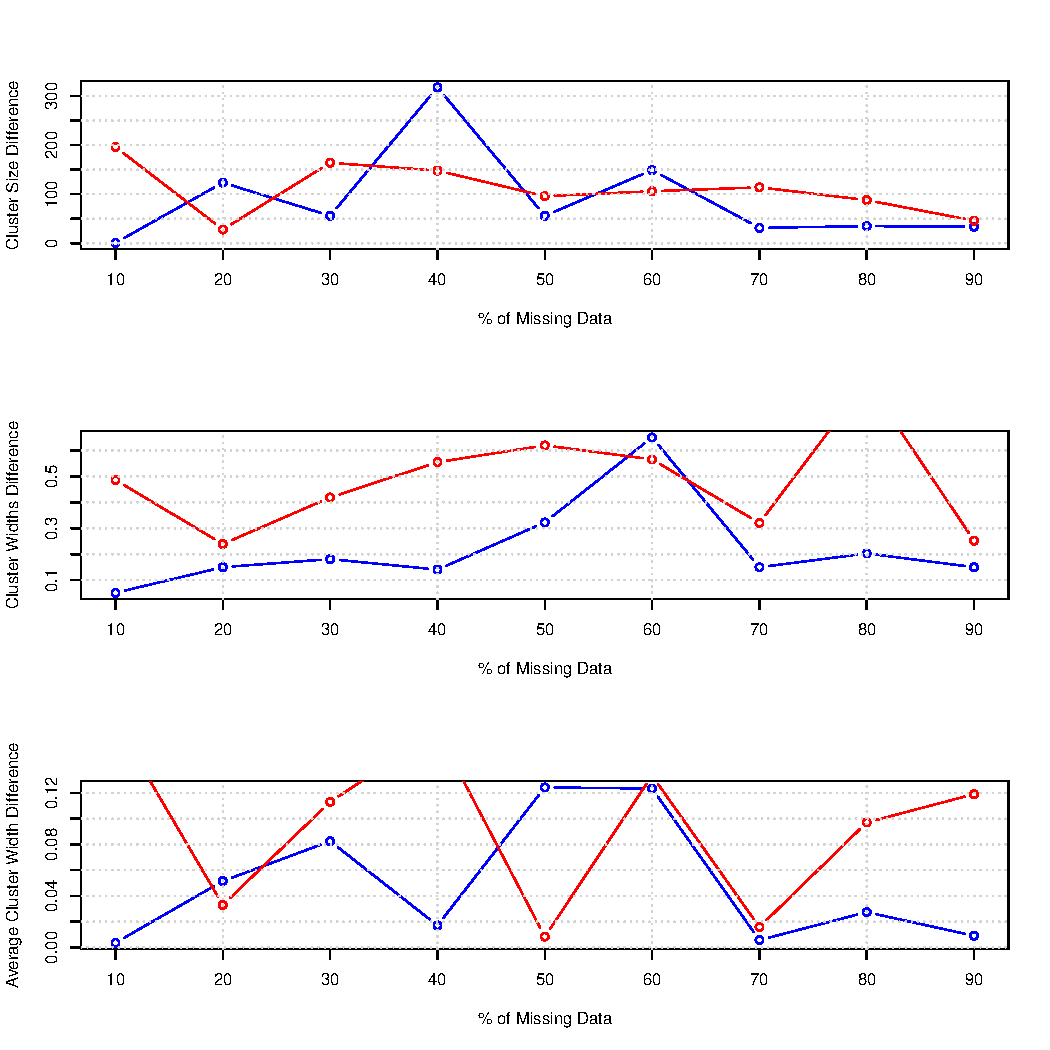
\includegraphics[width=\textwidth,height=0.9\textheight,keepaspectratio]{forestFires5} }
\end{frame}

\begin{frame}
  \frametitle{Forest Fires Outcomes}
  Outcomes:
  \begin{itemize}
    \item MICE works best when 20\% to 80\% of records contain missing values 
    \item If less than 20\% of the records have missing values, MICE might not be so effective. Could be as MICE needs lots of records with missing values to impute, more missing records means better prediction. 
    \item If a dataset has more than 80\% missing records MICE might not be so efficient, too much missingness could give false relationships and thus wrong imputation
  \end{itemize}
\end{frame}

\section{Mini-ABDN Summary}
\subsection{}

\begin{frame}
\frametitle{Missing Values in Mini-ABDN}
\centerline{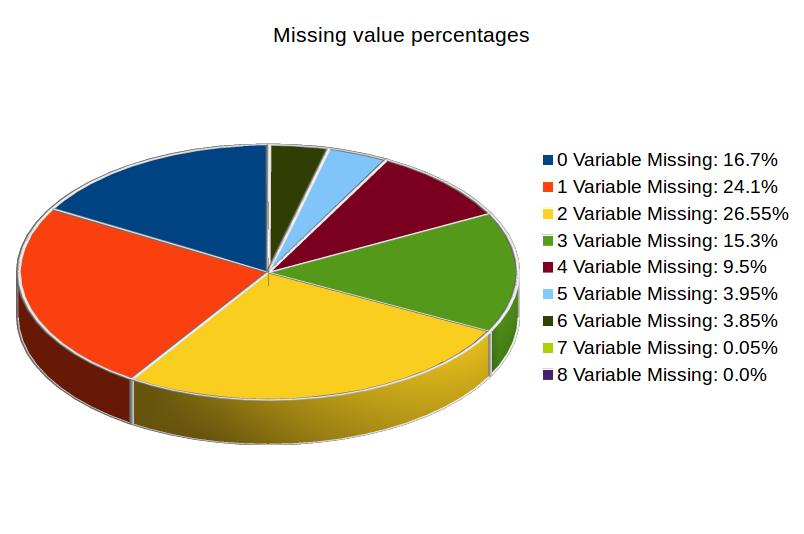
\includegraphics[width=\paperwidth]{missing-perc-equal}}
\end{frame}

% \begin{frame}
% \frametitle{Missing Values in Raw Data}
% \centerline{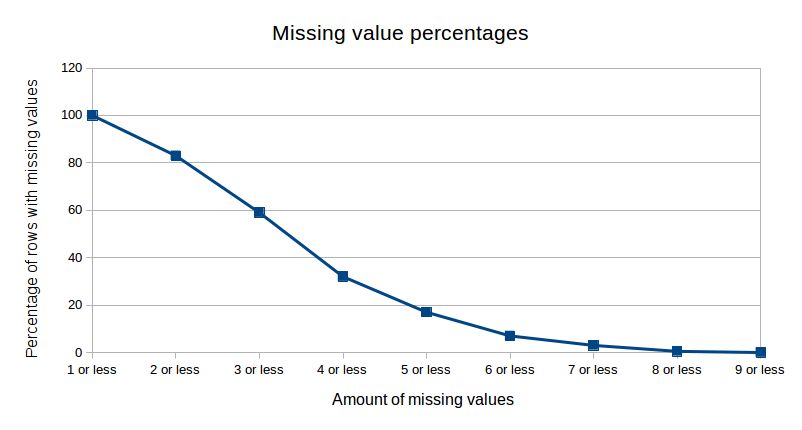
\includegraphics[width=\paperwidth]{missing-perc-min2}}
% \end{frame}

\begin{frame}
  \frametitle{Mini-ABDN}
  Mini-ABDN:
  \begin{itemize}
    \item 2000 records, 9 variables
    \item Mixed numerical and categorical variables 
    \item Can be used to find the amount of missing allowed for imputation
    \item Will allow increments of 10\% missing per records. 
    \item Chosen increments 20\% to 90\%
  \end{itemize}
\end{frame}

\begin{frame}
  \frametitle{Evaluate ABDN ctn.}
  % Distance Measure:
  % \begin{itemize}
  %   \item Clustering characteristics 
  %   \item 
  % \end{itemize}
  \center{ 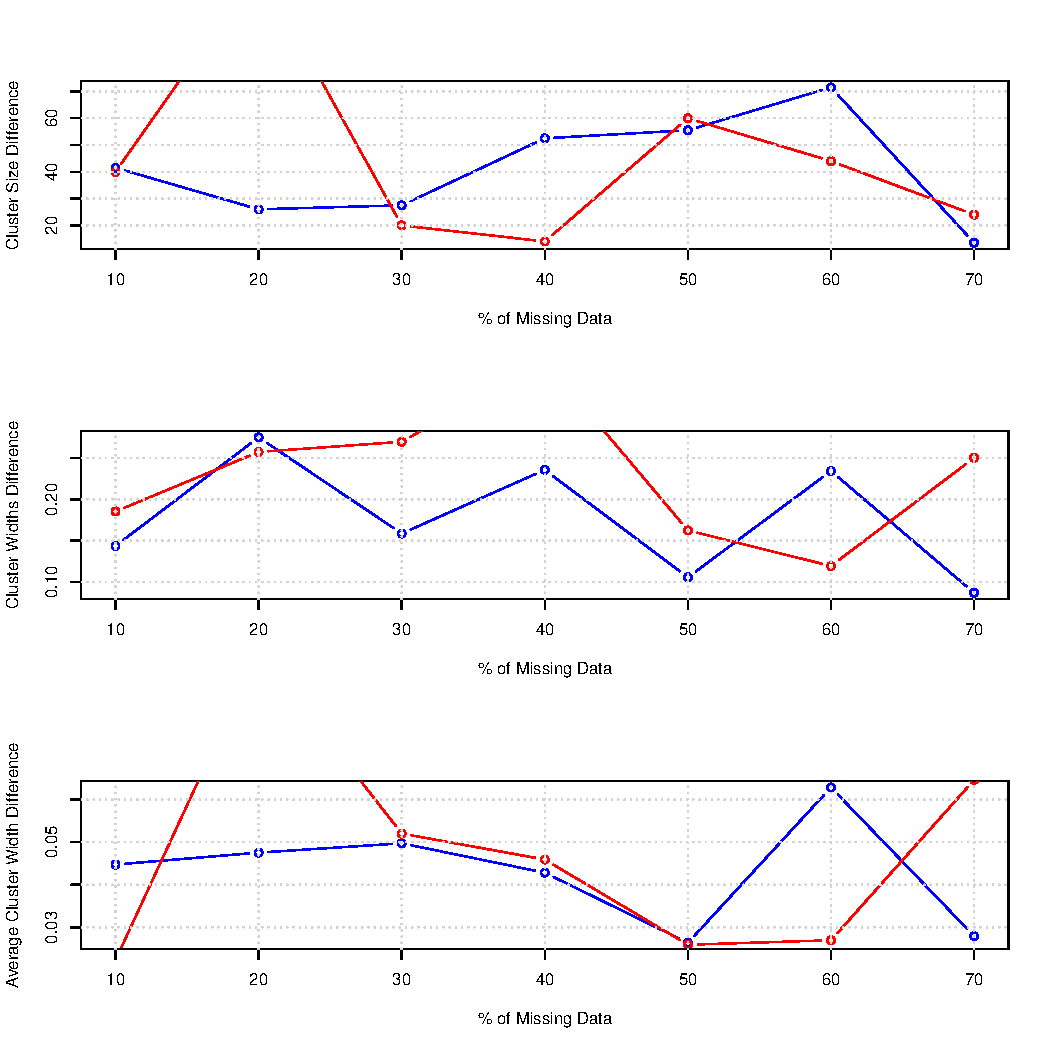
\includegraphics[width=\textwidth,height=0.9\textheight,keepaspectratio]{AMND} }
\end{frame}

\begin{frame}
  \frametitle{Evaluate ABDN ctn.}
  % Distance Measure:
  % \begin{itemize}
  %   \item Clustering characteristics 
  %   \item 
  % \end{itemize}
  \center{ 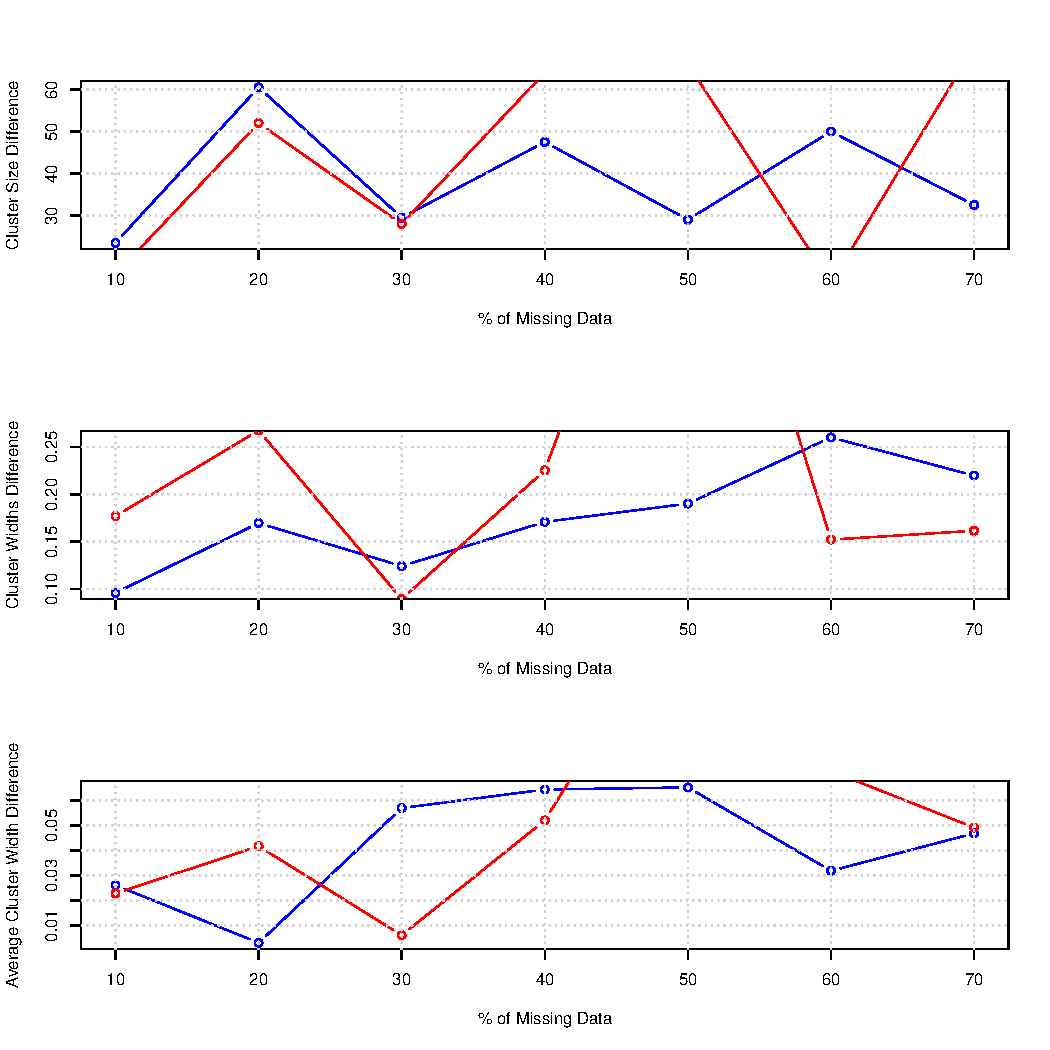
\includegraphics[width=\textwidth,height=0.9\textheight,keepaspectratio]{AMND2} }
\end{frame}

\begin{frame}
  \frametitle{Evaluate ABDN ctn.}
  % Distance Measure:
  % \begin{itemize}
  %   \item Clustering characteristics 
  %   \item 
  % \end{itemize}
  \center{ 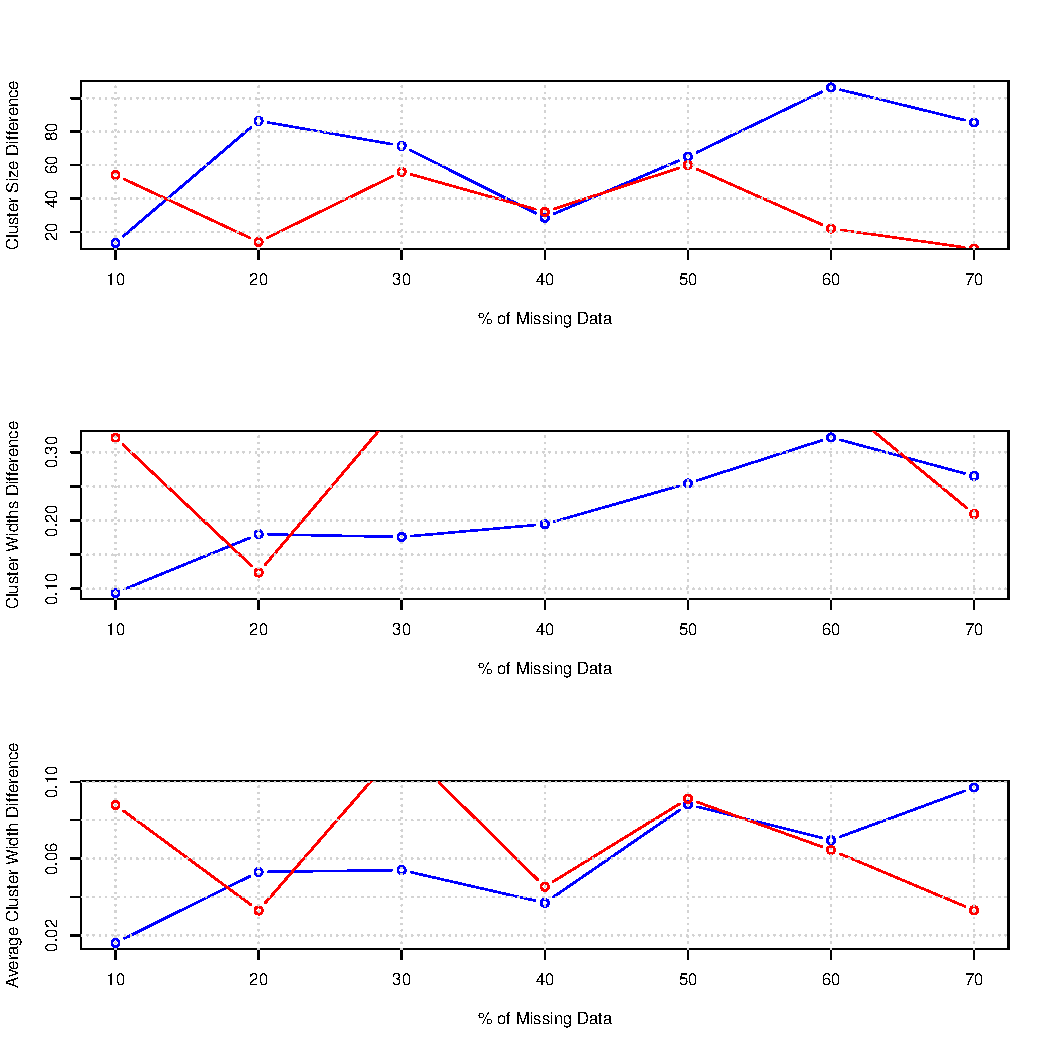
\includegraphics[width=\textwidth,height=0.9\textheight,keepaspectratio]{AMND3} }
\end{frame}

\begin{frame}
  \frametitle{Evaluate ABDN ctn.}
  % Distance Measure:
  % \begin{itemize}
  %   \item Clustering characteristics 
  %   \item 
  % \end{itemize}
  \center{ 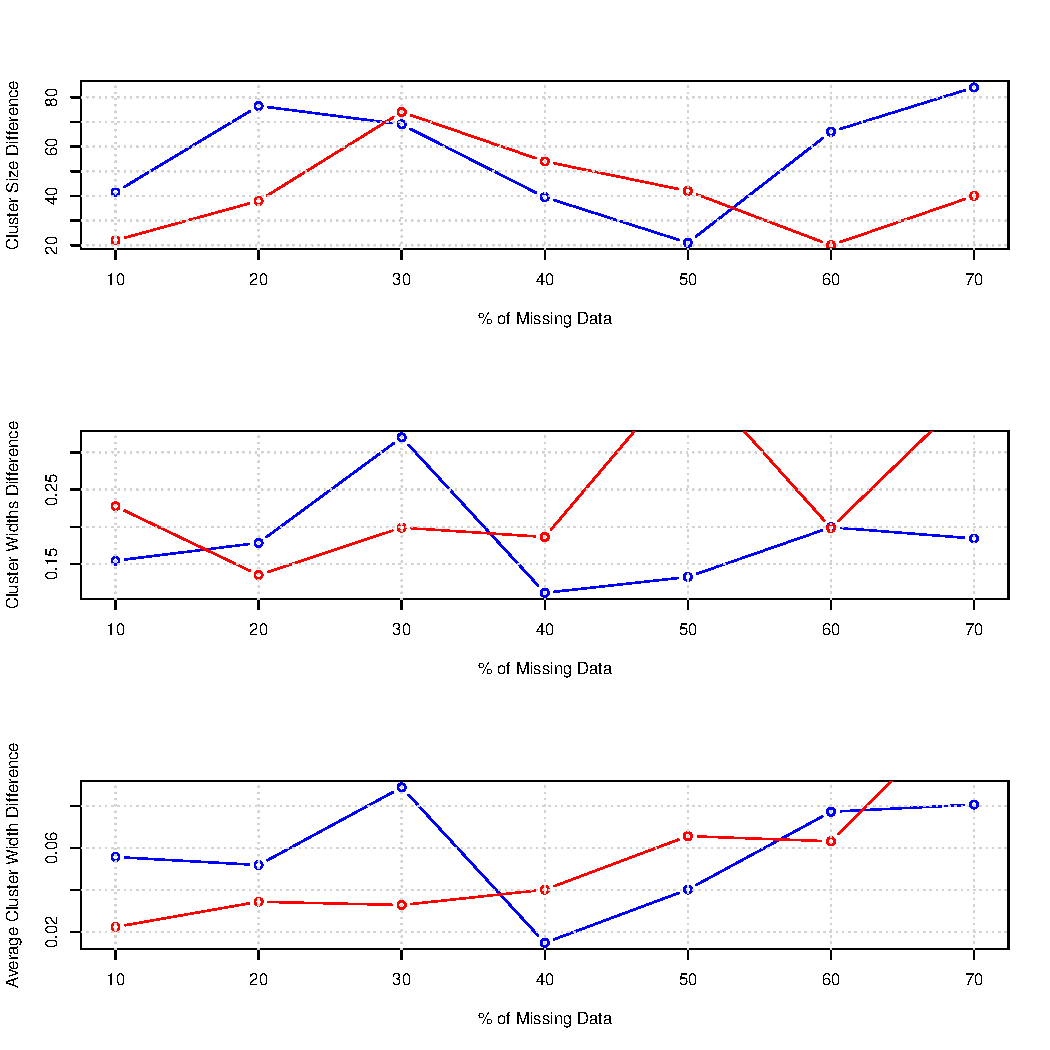
\includegraphics[width=\textwidth,height=0.9\textheight,keepaspectratio]{AMND4} }
\end{frame}

\begin{frame}
  \frametitle{Evaluate ABDN ctn.}
  % Distance Measure:
  % \begin{itemize}
  %   \item Clustering characteristics 
  %   \item 
  % \end{itemize}
  \center{ 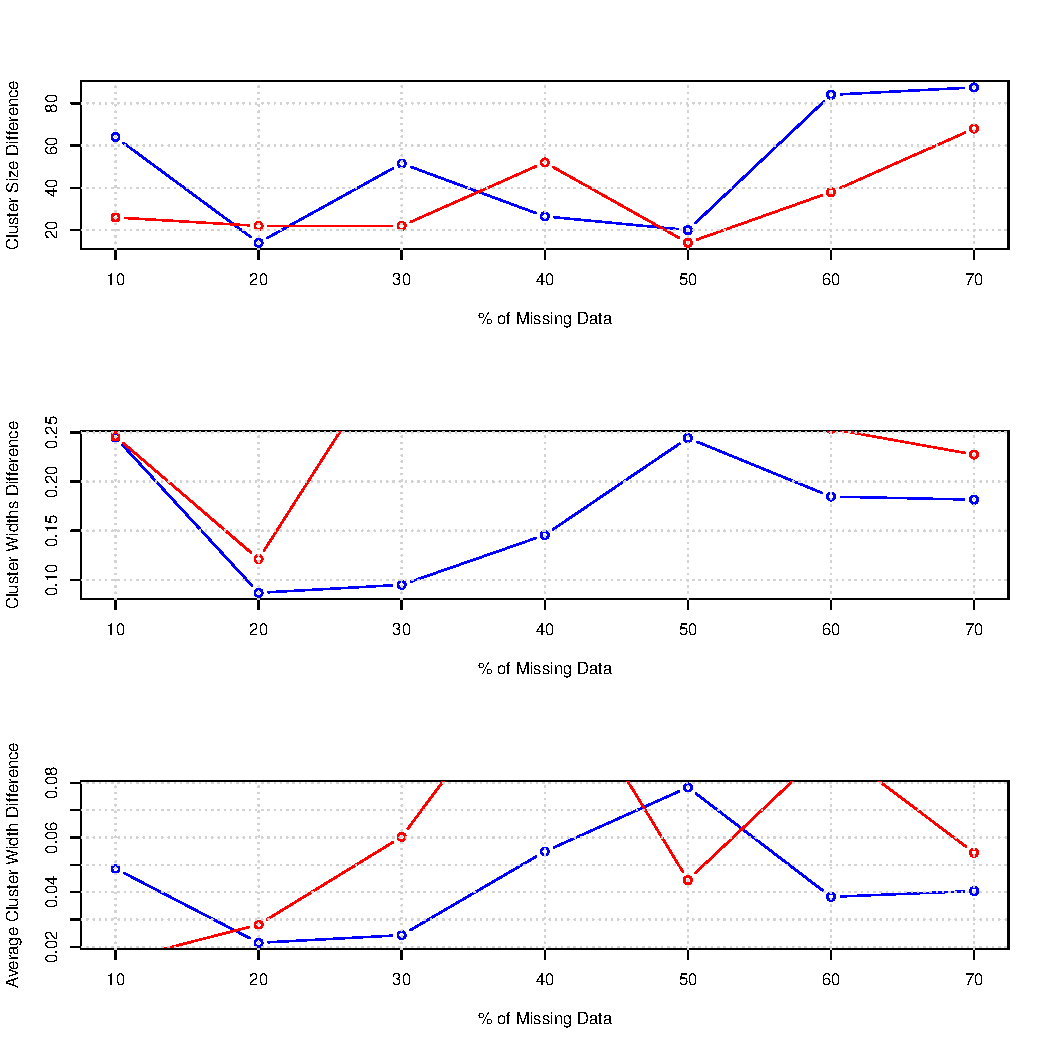
\includegraphics[width=\textwidth,height=0.9\textheight,keepaspectratio]{AMND5} }
\end{frame}

\begin{frame}
  \frametitle{Mini-ABDN Outcomes}
  Outcomes:
  \begin{itemize}
    \item MICE works best when there is 40\% to 80\% missingness
    \item If a dataset has less than 40\% missing variables on each record, might not be best to use MICE
    \item If a dataset has more than 80\% missing variabes on each records, only keep the records with less than 80\%
  \end{itemize}
\end{frame}

\section{Discussion}
\subsection{}

\begin{frame}
  \frametitle{Discussion \& Conclusion}
  Limitations
  \begin{itemize}
    \item Output is subjective 
    \item Some may over-interpret the results
    \item What if the complete subset is too small
  \end{itemize}
  Outcomes
  \begin{itemize}
    \item Optimised number of ignored records 
    \item Compare different imputation methods
    \item Optimize imputation features
  \end{itemize}
  To Consider
  \begin{itemize}
    \item Use modelling to verify the outcome 
    \item Use more imputation method
  \end{itemize}
\end{frame}


\begin{frame}
\frametitle{Thanks \& Questions}
\centerline{\Huge \myemph{Thanks for your attention!}}
\centerline{\Huge \myemph{Question \& Comments }}
\end{frame}

\end{document}


